%!TEX encoding=UTF-8 Unicode
\chapter{Case Study}
\label{chap:perf}

Optimizing a computation kernel is a complex tasks, it requires both a deep
understanding of the algorithm mechanics and of the machine that will execute
it. Lots of works have be done to optimize most usual linear algebra kernels
with the blas and lapack libraries. \DB{citations,gls} The task is even more
complex when it comes to optimizing a whole application, we first need to
identify the hotspots which means understand where and why the performances
are suboptimal. Then improving them is even more complex as the modifications
must be both efficient and understandable by developers not specialized in
\gls{HPC}, indeed cryptic optimizations are easily ignored. \DB{reformuler}
In this chapter, we present a case study on the performance optimisation of
\gls{SOFA}. It is organized as follow: first we present \gls{SOFA}, it's
specificities and previous attempt to parallelise or optimize it in
\sect{motivations}. Then we discuss the existing profiling tools that can
be used to analyze an application performances' in \sect{prof-tools}. After
that we detail our experimental methodology and discuss reproducibility
matters in \sect{expe-methodo}. Finally we present our analysis and first
conclusions in \sect{sofa}.

\section{Motivations}
\label{sec:motivations}


\gls{SOFA}~\cite{Allard07SOFA} is a simulation framework designed for
interactive and exact simulation as it aims at helping research in medical
simulation. Thus optimizing the performances of \gls{SOFA} is both mandatory
to reach interactive time and extremely complex as no approximation is
allowed.

\subsection{SOFA: a physical simulation framework}

\begin{figure}[htb]
    \centering
    \includegraphics[width=\textwidth]{simu-pipeline}
    \caption[The simulation pipeline]{The simulation pipeline}
    \label{fig:simu-pipeline}
\end{figure}


A simulation can be seen as a pipeline depicted in \fig{simu-pipeline}: we
start from an initial configuration were a set of objects are placed under a
force field. Then we have to resolve a system of equation to compute the next
position of each objects. The third step consist in detecting overlap between
objects and applying repulsing force to simulate the collision.  Finally the
result of these step is displayed (rendered) and we are back at the first
step. The time integration and the collision detection are the most costly
steps, there are many algorithms that allow to compute these steps efficiently
depending on the objects that are involved in them.

\begin{figure}[htb]
    \centering
    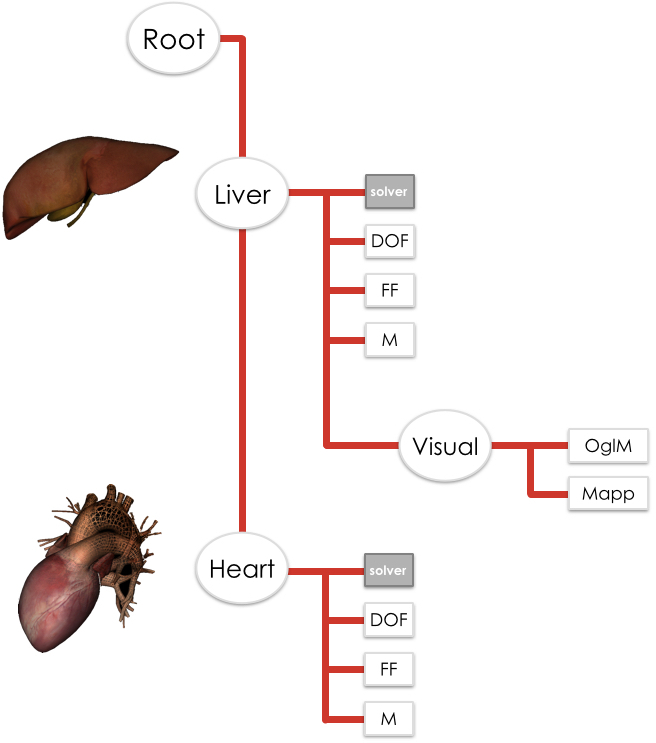
\includegraphics[width=\textwidth]{Sofa-graph}
    \caption[Example of SOFA scene graph]{SOFA representation of a scene with two objects: a liver and a
        heart. Each node of the scene can embed it's own set of solvers and
        visual representation.\\
        Image from SOFA documentation~\cite{SOFA16Sofa}.}
    \label{fig:sofa-tree}
\end{figure}

One of \gls{SOFA}'s main specificity is to have a multi-model representation
of each component: a simulation scene is represented as a graph, as shown in
\fig{sofa-tree}, each physical object is a node of the graph and can replace
the default solvers, collision detector and visual representation. This
hierarchical representation allows to manage dependencies between objects and
represent complex embedded objects~\cite{Nesme09Preserving,Faure11Sparse}.

\subsection{Previous work on SOFA parallelisation}

It is important to note that the main developers of \gls{SOFA} are  mostly
computer scientists with a physical or medical background but not specialized in
\gls{HPC}. Several efforts were made (by external developers) to parallelise
\gls{SOFA}, most of these efforts consist in optimizing one (or several)
algorithm(s) which, according to \gls{SOFA} developers is costly in time. For
instance, Everton Hermann proposed an efficient (sequential) collision
detection algorithm based on ray tracing and a parallelisation of this
algorithm~\cite{Hermann08Raytraced}. More recently, Julio Toss have been developing
several algorithms on \glspl{GPU} to improve the computation time of Voronoi
diagrams~\cite{Toss13Parallel,Toss14Parallel}. These diagrams are critical for
\gls{SOFA} indeed while they allow to simulate efficiently the propagation
of forces on heterogeneous materials~\cite{Faure11Sparse}, they generate a
considerable overhead before the simulation.

Yet the limitation of this approach is that it can only optimize part of the
code that are known to be slow. Furthermore \gls{SOFA} is a generic framework
used among other things to develop new simulation algorithm, this approach
does not provide any tool for \gls{SOFA} developers to parallelize their
algorithms by their own.

To overpass these limitations, E. Hermann exploited the hierarchy of the scene
graph to parallelize the time integration step using the \gls{KAAPI}
runtime~\cite{Gautier07KAAPI}. This runtime allows to provide several
implementations (\gls{CPU}, \gls{GPU} \ldots) for each task thus to reach
adaptive performances. Furthermore E. Hermann designed a parallelisation based
on domain decomposition for scenes with only a small number of
objects~\cite{Hermann09Interactive}.

While this approach seems to be more generic and easier to deploy it was never
actually used by \gls{SOFA} developers for several reasons: first of all they
are not specialized on parallelism thus not used to work with runtimes such as
\gls{KAAPI}. Second \gls{KAAPI} is a research runtime that evolve quickly,
therefore, the cost of maintaining code based on that runtime seems to
important to \gls{SOFA} developers.

Finally it appears that optimizing algorithm pointed out by
\gls{SOFA} developers is not enough as it can miss important part of the
execution and it does not help them to writing parallel code. Moreover
a structural parallelisation relying on a research runtime may be discarded by
them. Hence, we should acquire a deep knowledge of \gls{SOFA}
performances to identify hotspots and optimize the most important parts of
the code.

\section{Profiling tools}
\label{sec:prof-tools}

Performance analysis consists of to two steps: data collection and
presentation. The first step aims at extracting as much pertinent information
from an execution as possible, yet observing an execution is not free: it
takes time to count and record events thus it might change the application
behavior. Consequently, any analysis provide a trade-off between the amount of
data collected and the impact on the performance of the monitored application.
The second step is also challenging as the tools needs to understand which
data are pertinent and to present them in a meaningful way to the user.
Several tools were designed to address one or both of these challenges.

Performance counters, which were originally designed by \glspl{CPU} vendors to
debug their processors prototypes, allows to count events such as cache miss,
or branch miss-predict at a very low cost since they are hardware implemented.
They can directly be accessed using the \gls{Perf} driver which is part of the
\gls{Linux} kernel since version $2.6.31$. Yet as a result of their initial
aim, the available counters depends of the \gls{CPU} model and vendor,
furthermore it requires a deep knowledge of \glspl{CPU} mechanisms to
understand their meaning. Hence higher level library such as
\gls{PAPI}~\cite{Browne00Portable,Malony11Parallel,Weaver13PAPI} and
\gls{Likwid}~\cite{Treibig10LIKWID} to make it more convenient to access and
interpret performance counters. These libraries provides propose performance
groups and automatically computes comprehensive metrics. In addition they
allow to start and stop the counters during the execution to focus on critical
parts of the execution, which is useful once hotspot are identified, but can
lead to miss a part of the execution if used to early.

An other approach to make performance counters more understandable consist on
combining them with other informations obtained by hooking libraries calls
(system calls, C standard library, \gls{MPI}, \gls{OpenMP} \ldots). Such hooks
can be deployed either by overwriting libraries calls at runtime with
\texttt{LD\_PRELOAD} hack, or by using binary instrumentation libraries such
as \gls{Intel} \gls{Pin}~\cite{Luk05Pin} or Dyninst from the Paradyn
Project~\cite{Miller95Paradyn}. The second method is more flexible and usually
allows higher level data collection, yet it is more intrusive thus it might
impact the behavior of the studied application. Simulators such as
\gls{SimGrid}~\cite{Casanova14Versatile} can be used to overpass these
limitations, still they are more complex to install and use thus less likely
to be adopted by developers from other fields than \gls{HPC}. Several tools
such as \gls{HPCToolkit}~\cite{Adhianto10HPCTOOLKIT},
\gls{PARAVER}~\cite{Pillet95PARAVER}, \gls{TAU}~\cite{Shende06Tau},
\gls{MAQAO}~\cite{Djoudi05MAQAO}, \gls{AMD}
\gls{CodeXL}~\cite{AMD16CodeXL} (the successor of \gls{AMD}
\gls{CodeAnalyst}~\cite{Drongowski08introduction}) and \gls{Intel}
\gls{VTune}~\cite{Reinders05VTune} combines several of these methods to
collects traces.

When it comes to presenting performance traces in a readable way, we can split
these tools in three groups: the first one only provides textual traces and
let the user extract pertinent informations from them. This groups includes
the \gls{Perf} driver, \gls{Likwid} and \gls{PAPI} library as well as several
\glspl{Pintool}. Such traces are very useful for small applications as they
does not require complex tools to be read, furthermore they are usually easy
to parse thus one can build more complex visualisation upon it. Tools from the
second group, that includes\gls{VTune}, \gls{CodeXL} tries to present data in
a more readable way, usually a set of tables and few plots. Moreover they
highlight values that seems to be pertinent (for instance cache miss above a
reasonable threshold) to help the user focusing on important parts. Finally,
while tools like \gls{MAQAO}, \gls{HPCToolkit} and \gls{PARAVER} propose
visualisation similar too the second group by default, they also provides
simple \glspl{API} to design new visualizations or import external traces.
\gls{Framesoc}~\cite{Pagano13Trace} is very similar to the previous tools, the
main difference is that it is designed for trace management and analysis, thus
it does not provide any way to collect traces but it is able to import traces
from several tools an describe them with a generic representation. It allows
to store traces and navigate easily through different visualizations.

To conclude, many tools were developed to monitor an application's
performance, the best tool depends of the kind issue we are looking for and
the application we are monitoring. Most of the tools discussed here are based
on performance counters and therefore focus on the \gls{CPU}'s point of view.
In our specific case, we are studying a complex application, yet we are in
contact with the developers of \gls{SOFA} thus the can give us hints on the
important parts and the kind of issue we should look for. Therefore low level
tools such as \gls{Likwid} are well suited as they allow both to compute
pertinent metrics and to focus on different part of the application.

\section{Experimental Methodology}
\label{sec:expe-methodo}

While in other domains such as biology experiments takes a large amount of
time and money, they are almost inexpensive and can be designed very quickly
in computer science. As a results, we computer scientists, are not used to
take the time to design correct experiments trying to minimize bias and using
the right tools. Furthermore as hardware and software evolves very quickly we
usually does not bother to re run and verify the results presented previous
studies while it is the best way to spot bias or confirm the validity of an
experimental claim.

In this section we first introduce why reproducibility matters and how people
have try to reach it in \gls{HPC}, then we present the methodology we have
developed during this thesis to make our experiment as reproducible as
possible.


\subsection{Reproducible research}

Measurement bias is a widely known phenomena in scientific communities and is
analyzed in most fields. Still in \gls{HPC} the only thing we usually do to avoid it
is to run a large number of experiments hopping that if we have enough
observations on several configurations the measurement bias will be
negligible. Mytkowicz et al.~\cite{Mytkowicz09Producing} highlighted several
way to introduce significant measurement bias in computer science experiments
without noticing it, showing that measurement bias is commonplace and
unpredictable in our field.

As measurement bias is unpredictable even when we follow the best practices
the easiest way to deal with it is to reproduce the study published by other
team and confirm or invalidate their results. While this is done in every
scientific fields, it is not common to publish about experiment reproduction
in \gls{HPC}.

A previous study~\cite{Collberg15Repeatability} tried to evaluate how
reproducible the experiment presented in computer science article are. To do
so, they focused on the capacity to build the experimental code and evaluated
$601$ articles published in “top ACM conferences and journal”. From these
$601$ articles they were only able to build the environment of $217$ articles.
Moreover it took more than half an hour to build $64$ of these papers and $23$
other required the intervention of the authors.

At this point we need to define precisely reproducibility, for the remaining
of this thesis, except if specified otherwise, we will use the definition
proposed by Dror G. Feitelson~\cite{Feitelson15From}:

\begin{quote}
    Repeatability concerns the exact repetition of an experiment, using the
    same experimental apparatus, and under the same conditions.

    Reproducibility is the reproduction of the gist of an experiment:
    implementing the same general idea, in a similar setting, with newly
    created appropriate experimental apparatus.
\end{quote}

It is nearly impossible to repeat an experiment in the exact same conditions
as many exterior factors, such as the machine room temperature or the network
usage done by other users  \DBm{Citations ? Demander a Arnaud ?} on the same cluster, might impact the measured
performances.
Still it is possible to repeat an experiment in similar conditions: someone
who runs the same experiments two different days on the same machines can
expect to obtain similar results. Several tools can helps use making
experiments more repeatable for instance by running our experiment on a shared
platform such as grid5000~\cite{Cappello05Grid5000} we can hope that other
people might access to the same set of machines. Moreover deploying a custom
environment on these machines allow to control and distribute the set of
installed libraries. Kameleon~\cite{Ruiz15Reconstructable} go even
further as it allows to describe an environment as a recipe thus makes it easy
to check the version of a library or replace it.

To reproduce an experiment it is important to understand how it has been
designed and how it evolves from the first version to the results presented in
the paper. Stanisic et al.~\cite[Chapter~4, p31-44]{Stanisic15Reproducible}
described an experimental workflow based on \emph{git} and \emph{emacs orgmode}
to keep track of these evolutions and make easy for someone to understand it.
One of the main drawback of this workflow is that it is not suitable for
experiment which generate huge ($\ge$\SI{500}{Mib}) trace files as git is not
designed to handle such files.

Several tools were designed to conduct experiments in computer science still
they are not designed for \gls{HPC} and using them in our context would
require some adjustments. A more complete survey can be found
in~\cite[Chapter~3, p17-19]{Stanisic15Reproducible}

\subsection{Experimental workflow}

We design experiments to answer simple questions such as ``Is my tool more
efficient than the existing ones'', obviously this formulation is too vague to
be answered scientifically. We first need to find a set of relevant state of
the art tools and then decide and on which configurations we are going to do
the comparison. This means choosing a set of benchmarks representing real life
applications, one or several credible experimental machine(s). Finally we must
determine a set of metrics that we can measured accurately to evaluate the
efficiency of the tools.

\begin{figure}[htb]
    \centering
    \includegraphics[width=\textwidth]{exp-tikz}
    \caption{Experimental pipeline}
    \label{fig:exp-pipeline}
\end{figure}

All these choices form a high level \emph{experimental plan}: it contains all
the information required to reproduce the experiment but not to repeat it.
Indeed it miss the code that actually execute the experimental plan.
We can see an experiment as a pipeline that flow from this plan to the final
human readable results as described in \fig{exp-pipeline}. This pipeline is
composed of three steps: the experimental plan that produce a (usually) huge
set of data and meta data, the first one are meant to be used during the
analysis while the second are only generate to find issue in the experiment or
additional information to repeat it. Then comes the raw analysis that extract
pertinent information and compute metrics from the raw data. The results of
this step are usually easy to parse for a computer but not human friendly.
Thus the last step is there to present these data in a readable way.

Yet it is easy to present data in a tendentious way that reflects more our
expectations than the reality without even noticing it, we call this the
\emph{experiment designer bias}\DBm{Ref ?}. To limit this bias,
it is very important to design carefully the whole analysis before running the
actual experiment and test the visualisation on a filler set of data.
Furthermore, adding comments to the visualisations about what they mean and
what we expect to see can help avoiding this bias. Technologies such as
\texttt{R-markdown},\texttt{Jupyter Notebook} (anciently known as IPython
Notebook) or \texttt{Emacs Orgmode} are great help to produce reproducible
experiments.

\subsubsection{Methodology}

\paragraph{Preparing an experiment:}

In this thesis, we ran two types of experiments: the fist one aims at
analysing the behavior of one application (mostly \gls{SOFA}) while the second
one aims at comparing trace collection tools. For both analysis we need to
find a set of \emph{benchmarks} conduct our experiments, but the signification
of this term is slightly different for the two cases. In the first case, a
benchmark is an input for the studied application and the set of benchmarks
used should be defined with the developers of the application to cover the
code that they want to improve. While in the second case it means a set of
applications, for this need, we use the \gls{npb}~\cite{Jin1999} which allow
to cover a large set of applications from simple computational kernels to real
life applications. Yet to compare several analysis tools, a set of benchmarks
is not a sufficient input as these tools usually provides a large set of
parameters allowing to modify their behavior, thus we must evaluate each tool
under at least two set of parameters: the default and a tuned version with a
set of parameters optimized for the results we are measuring.

Once the benchmarks are chosen, we need to decide of one machine or a set of
machines on which we will run the experiment. This step is crucial as
computers architectures are getting more and more complex \DB{Ref partie 2.1
?} and applications are (usually) designed for one type of machines.
Furthermore some tools (such as \gls{Pin}\DBm{Citation ?}, \gls{PEBS}, \gls{IBS}) are vendor
specific or optimized for some architecture. Thus we must find machines that
allow to do our study in a relevant situation and fair to the tools and
libraries used.

Finally we need to find some relevant metric(s) to answer the question(s) that we
are trying to answer with our experiment. These metrics should remain as
simple as they will be interpreted by humans. Yet they must also cover every
aspects that we are studying. A complete set of simple measurable metrics is
often easier to understand that one complex metric that provide an overall
score in an unknown unit. Still simple ratios and percentages can make an
analysis more reproducible for instance an execution time is significant only
for a very specific configuration on one machine, while speedups and overheads
can be compared more easily.


\paragraph{Writing the experiment scripts:}

It is crucial that any step of the experiment from the deployment of the
environment to the final analysis is properly scripted in a language that can
be understood by an other developer. Any manual step can make the experiment
hard to reproduce and an obscure code might make it hard to change some
parameters.

Furthermore the traces generated by an experiment must be self explanatory or
at some point they will only be a (large) set of meaningless bytes on a hard
drive. To do so it is important to keep together the data and both the scripts
that generated it and the one that allows to interpret its. To do so, all our
experimental scripts starts the same way: they create a new directory that
will hold the traces, copy themselves and all the scripts which are on their
directory inside it. Then they duplicates their output to a file in this
experimental directory and Log every sensible meta data such as the
command that started the experiment, the machine name, its topology, \gls{OS}
the environment variables, the status of every dependencies (git version, diff
etc.). Such informations can be a great help to someone trying to reproduce
the experiment or to verify that the experimental condition are not biased.

The actual execution of the experiment consist of a set of runs, to limit the
impact of external noise, it is a good practise to randomize these runs.
Therefor our experimental scripts generate the list of runs that should be
executed shuffle it and then execute it run in a randomized order. A run
consist of three step: a pre command that can set specific values for the run,
the actual command that execute the benchmark and the post command that can
save data, might compute metrics and must restore the normal state. Note that
the first and last steps are not mandatory. Each of the commands executed by
these 3 steps are printed before execution thus logged.

At the end of the day our experiment have produced a huge set of data that we
can divide on two categories: the meta data that are useful for debugging and
reproducibility and the raw results that will be filtered to then be analyzed.
The parsing step is designed only to extract data from the traces so the
analysis scripts can work on clean results, we avoid to do any statistic
during this step.

Finally for the analysis \texttt{R} provides a large set of reliable statistic
analysis libraries and technologies such as \texttt{R-markdown} or
\texttt{Orgmode} allows to mix analysis code and results with comments. These
technologies allow to produce a standalone result (as a pdf or as a webpage)
that contains the original questions, our assumptions, the results and plots,
and our observation on these results.

\paragraph{Distributing the experiment:}

Trying to compile a badly documented code can be painful and time consuming,
the same problems occurs when it comes to reproduce experiment. Thus the
distribution of the experiment traces and script must be considered carefully.
To reproduce an experiment with need the scripts that run it, a description of
the machines and/or the virtual environment that is deployed and a link to the
right version of each tool, applications and benchmarks used during the
experiment. Several services such as Github, Bitbucked, and Gitlab \DBm{Urls ?}
host freely code repositories, furthermore \glspl{VCS} such as Git and
Mercurial \DBm{Citations ?} allow to track easily dependencies with a system
of submodules, therefore they are well suited for experiment distribution.
Finally an effort must be done on the documentation to help the user
understand why the experiment is designed, how it works and where (on which
machines) we should run it.

Distributing the experiment results can be more tricky as these files can be
quite heavy and code repositories are usually not designed to handle large
files. While the experimental repository allows to reproduce the whole
experiment, the trace distribution is useful to reproduce only some specific
steps of the analysis, thus we distribute to set of files corresponding to the
two analysis steps depicted in \fig{exp-pipeline}. The first one contains all
the files generated by the experiment and the scripts to run that analysis.
This distribution can be quite heavy (around \SI{100}{Gib} for some of our
experiments) but allows to redo the whole analysis, compute new metrics or
look for additional informations in the meta data. At the opposite, the second
one only contains the filtered results and the scripts that generate the
plots, it allows to redo the statistical analysis exploring the data with a
different approach. Furthermore this trace usually contains more plots and
data than a published article that have to fit a certain amount of pages. Such
traces can be distributed using specialized large file hosting services such
as Renater File Sender, or Zenodo.\DBm{Url, Citation ?}


\section{Analysis}
\label{sec:sofa}

In this section, we present first the experiment designed to produce a
performance analysis of \gls{SOFA}, then we discuss the obtained result on the
possibility of improvements.

\subsection{Experiments}

\begin{itemize}
    \item  Note: Methodo not exactly as explained above, as it get more
        precise with time: no only publication for reproducibility / no
        deployable environment
    \item Parallelisation of SOFA => omp vs sequential
    \item Configuration
        \begin{itemize}
            \item Naskapi
            \item SOFA last version
            \item 4 simulation scenes specially crafted by SOFA main devs
            \item Focus on few functions pointed by the devs
        \end{itemize}
    \item Metrics
        \begin{itemize}
            \item Overall simulation time
            \item Time in each functions
            \item L2/L3 bandwith / data volume
            \item Mem Bandwith / data volume
            \item Idle time
        \end{itemize}
    \item Expected behavior:
        \begin{itemize}
            \item Most time should be spent in the observed functions
            \item Parallelisation should be at least as bad as sequential
            \item Omp should increase data volume in L3 cache but also
                bandwith
        \end{itemize}
\end{itemize}

Voir Wiki/Meetings/CR\_Reu\_Sofa\_20140326.wiki

voir:
\begin{itemize}
    \item /home/david/Work/Sofa/expe/FlexibleLikwidPerfctr/MarkerFullTree\_140331\_1650/analyse.html
        \begin{itemize}
            \item LinearRigidAndAffine
                \begin{itemize}
                    \item OMP slower then seq
                    \item SeqMat: all level, BW and data volume loss
                    \item ApplyJT vec:
                        \begin{itemize}
                            \item Mem: More volume, comparable (low) BW
                            \item L3: More Volume, More BW comparable increase
                            \item L2: More volume, comparable BW (check
                                numbers)
                        \end{itemize}
                    \item ApplyDJT:
                        \begin{itemize}
                            \item MEM: Less BW (more than X2), Less Data (less than x2)
                            \item L3: Less BW (x2), More Data, x2
                            \item L2: Less BW (more than x3), Comparable data
                            \item For other scenes, BW increase at all level
                        \end{itemize}
                \end{itemize}
        \end{itemize}
\end{itemize}

\DB{Do Figure for each level, ApplyDJT, BW and Volume, OMP and Seq,
    LinearRigidAndAffineFrame, linearQuadraticFrame. And figure simu time OpenMp vs
Seq for RigidAndAffineFrame and LinearQuadraticFrame}



\subsection{Results and Discussions}


ApplyJ Vec:
    + Moins de data Mem => meilleur util cache
    + plus de data en cache (L3 et L2) avec plus de bande passant => bien,
    yet, bande passante jamais maximale => faux partage ?

\DB{Need memory oriented tools, improve the methodology}
